\lab{Plotting With matplotlib and Mayavi}{Plotting}
\objective{Introduce some of the basic plotting functions available in matplotlib and Mayavi.}
\label{lab:Matplotlib_and_Mayavi}

\section*{2-D plotting with \li{matplotlib}}
The Python library \li{matplotlib} will be our primary tool for creating 2-D graphs in this text. This lab introduces the basic features of \li{matplotlib}; for more information, visit the documentation at \url{http://matplotlib.org}.

To begin, import \li{pyplot} from \li{matplotlib}.
\begin{lstlisting}
from matplotlib import pyplot as plt
\end{lstlisting}

\subsection*{Line plots}
The function call \li{plt.plot(x, y)} takes two 1-D NumPy arrays, \li{x} and \li{y}, and plots the points \li{(x[i], y[i])}, connecting them with straight lines.

For example, this code plots $y=e^x$ on the interval $[-2,3]$. The output is in Figure \ref{fig:exp_plot}.
\begin{lstlisting}
import numpy as np
# Create an array of 501 evenly spaced points in [-2,3].
x = np.linspace(-2, 3, 501)
y = np.exp(x)
plt.plot(x, y)
plt.show()
\end{lstlisting}


\begin{figure}
\centering
\begin{subfigure}[t]{.49\textwidth}
\centering
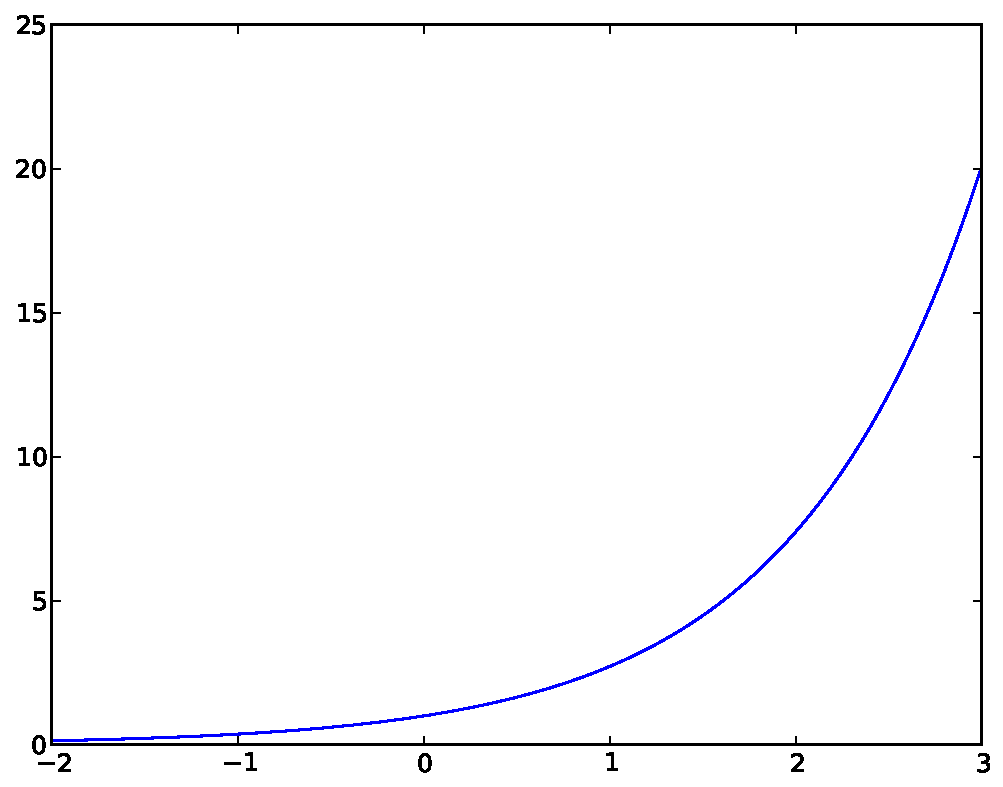
\includegraphics[width=\textwidth]{exp_plot.pdf}
\caption{A graph of $e^x$.}
\label{fig:exp_plot}
\end{subfigure}
\begin{subfigure}[t]{.49\textwidth}
\centering
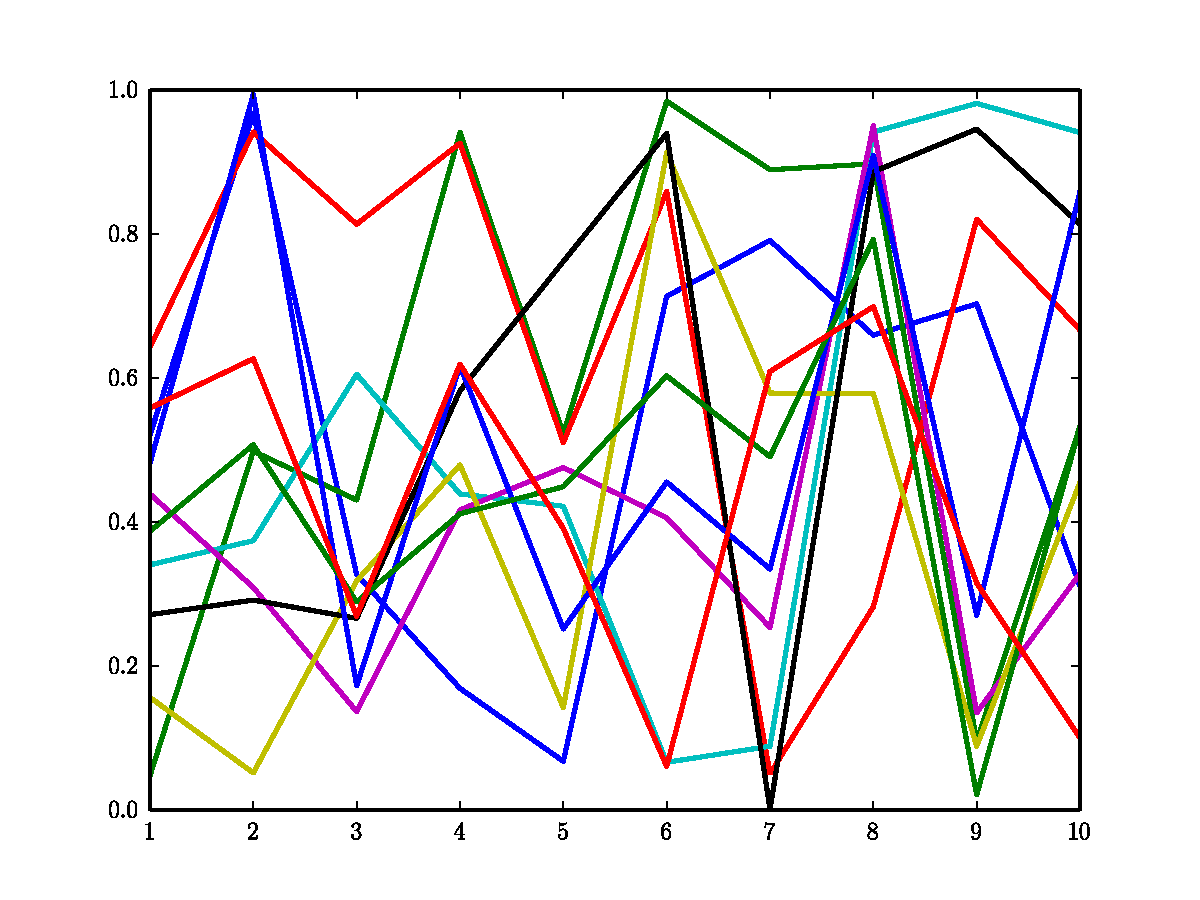
\includegraphics[width=\textwidth]{statemachine.pdf}
\caption{A graph of ten lines with randomly generated $y$ values.}
\label{fig:statemachine}
\end{subfigure}
\caption{Plots created with \li{plt.plot()}.}
\label{fig:lineplots}
\end{figure}


All calls to \li{plt} functions will modify the same figure until you call \li{plt.show()}. 
The function \li{plt.show()} displays the current figure and resets the system, so that the next call to a \li{plt} function modifies a new figure. 

We can take advantage of this system to plot multiple lines on the same axes.
For example, the following code plots ten lines, each with random values at integers from 1 to 10. 
The output is in Figure \ref{fig:statemachine}.
\begin{lstlisting}
x = np.linspace(1, 10, 10)

# Create a 10x10 array of uniformly distributed values in [0,1).
y = np.random.rand(10, 10)

# Plot each row of y
for row in y:
    plt.plot(x, row)
plt.show()
\end{lstlisting}

Alternatively, we can produce the same graph with a single call to \li{plt.plot()}.
\begin{lstlisting}
plt.plot(x, y[0], x, y[1], x, y[2], x, y[3], x, y[4], x, y[5], x, y[6], x, y[7], x, y[8], x, y[9])
plt.show()
\end{lstlisting}



\begin{comment}
\begin{problem} Plot the function $\sin(x)$ from $0$ to $2\pi$ with a red dashed line.
Then plot the function $\cos(x)$ on the same domain with a blue dotted line.
Implement both with a single call to the \li{plot()} function.
Information on how to do this can be found in Appendix \ref{mpltables}.
\end{problem}
\end{comment}

\begin{comment}
There are also many functions that we may use to set different values in
the plotting environment. A few examples are shown in Table
\ref{mpl:useful_functions}.

\begin{table}
\begin{center}
\begin{tabular}{|l|p{6cm}|p{4cm}|}

    \hline

    Function & Description & Usage\\

    \hline

    \li{annotate} & adds a commentary at a given point on the plot &
    annotate('text',(x,y))\\

    \li{arrow} & draws an arrow from a given point on the plot &
    arrow(x,y,dx,dy)\\

    \li{axhline} & draws a horizontal line at y from xmin to xmax &
    axhline(y=0, xmin=0, xmax=1)\\

    \li{axvline} & draws a vertical line at x from ymin to ymax &
    axvline(x=0, ymin=0, ymax=1)\\

    \li{axhspan} & draws a rectangle from xmin to xmax and ymin to ymax,
    if no xmin and xmax are given it goes across the plot &
    axhspan(ymin, ymax, xmin=0, xmax=1)\\

    \li{axvspan} & draws a rectangle from ymin to ymax and xmin to xmax,
    if no ymin and ymax are given it goes across the entire plot &
    axvspan(xmin, xmax, ymin=0, ymin=1)\\

    \li{figlegend} & place a legend in the plot & figlegend(handles,
    labels, loc)\\

    \li{grid} & add gridlines & grid()\\

    \li{text} & add text at a given position on the plot &
    text(x,y,'text')\\

    \li{title} & add a title to the plot & title('text')\\

    \li{xlim} & set the x limits, returns current limits if no arguments
    are given & xlim(xmin,xmax)\\

    \li{ylim} & set the y limits, returns current limits if no arguments
    are given & ylim(ymin,ymax)\\

    \li{xticks} & set the location of the tick marks on the x axis,
    returns current locations if no arguments are given & xticks(x)\\

    \li{yticks} & set the location of the tick marks on the y axis,
    returns current locations if no arguments are given & yticks(y)\\

    \li{xlabel} & add a label to the x axis & xlabel('text')\\

    \li{ylabel} & add a label to the y axis & ylabel('text')\\

    \hline

    \end{tabular}
    \end{center}
    \caption{Some Functions to Set Plotting Options}
    \label{mpl:useful_functions}
    \end{table}

	\end{comment}
	
\begin{problem}\label{prob:lineplot}
Plot the curve $1/(x-1)$ on [-2,6].
Do the following to your plot:

\begin{enumerate}
\item The function \li{plt.plot()} will make the curve look continuous at $x=1$. 
Plot the two sides of the curve separately (still with a single call to \li{plt.plot()}) so that the graph looks discontinuous at $x=1$.
\item Plot the curve with a line that is magenta, dashed, and thick (see Appendix \ref{mpltables}).
\item Change the range of the $y$-axis to be $[-6, 6]$.
\end{enumerate}
Your final plot should look like Figure \ref{fig:problem2}.

\begin{figure}[H]
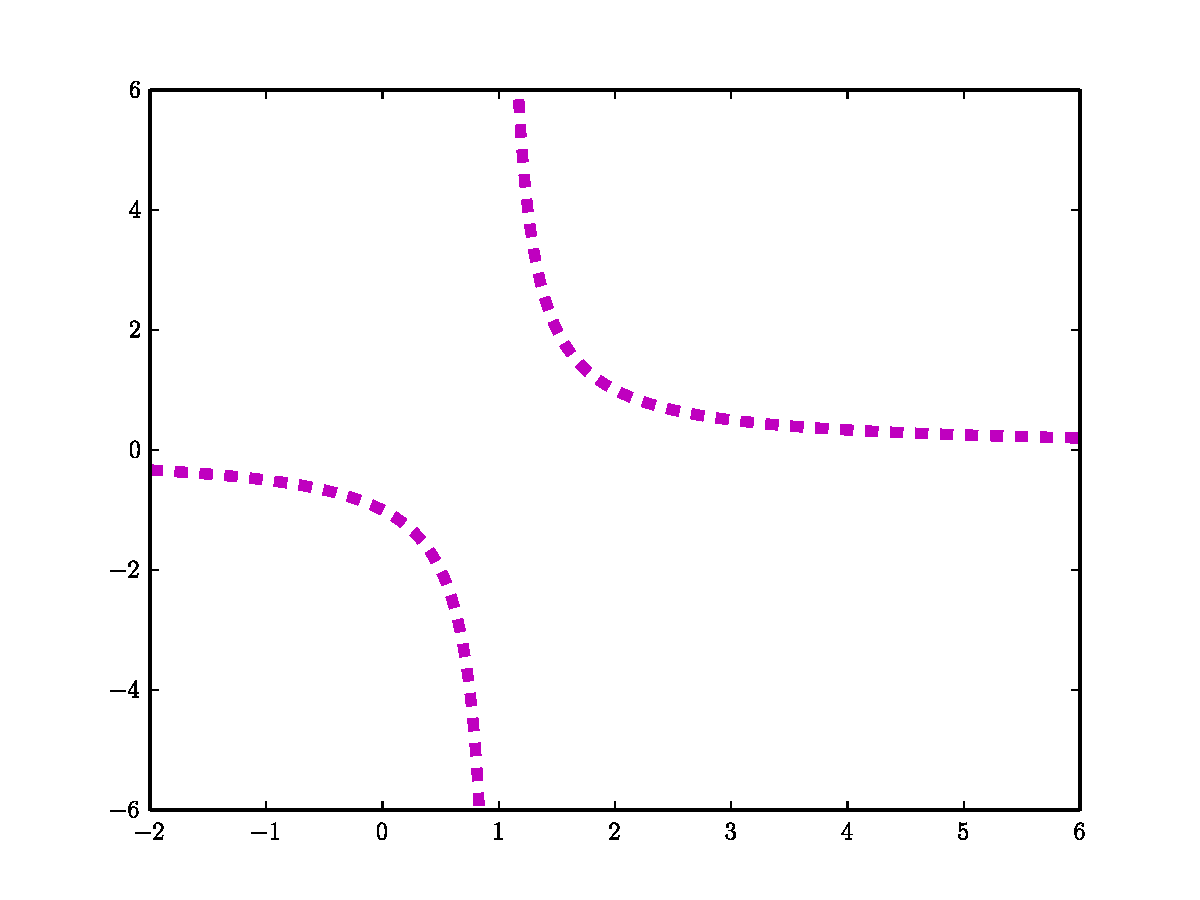
\includegraphics[width=.7\textwidth]{soln2.pdf}
\caption{Correct output for Problem \ref{prob:lineplot}.}
\label{fig:problem2}
\end{figure}
\end{problem}

\begin{comment}
\begin{problem} Plot the curve $\sin(x)\frac{1}{x+1}$ from $0$ to $10$.

Use blue shading under the curve when it is positive and red when it is negative (you may want to consider using the \li{fill_between} command.
Make the line dotted.
Label the x-axis ``x-axis'', the y-axis ``y-axis'',and the plot ``My Plot''.
Enable the grid lines.

Finally, use the \li{scatter} command to include a scatter plot of half of the value of the function at each of its maxima and minima in the range.
Display these points as upward-pointing triangles.
Don't forget to make sure the x limits of the plot are still 0 and 10.

\emph{Helpful Hint}: Since you are working with arrays of discrete values, you will want to find the index values where your $x$ and $y$ values are closest to the actual maxima and minima. As you work, consider the following:
\begin{itemize}
\item How would you manually find maxima and minima of a function?
\item How could you do something similar with your $x$ and $y$ arrays?
\end{itemize}
Your plot should look like the figure below.

\begin{figure}[H]
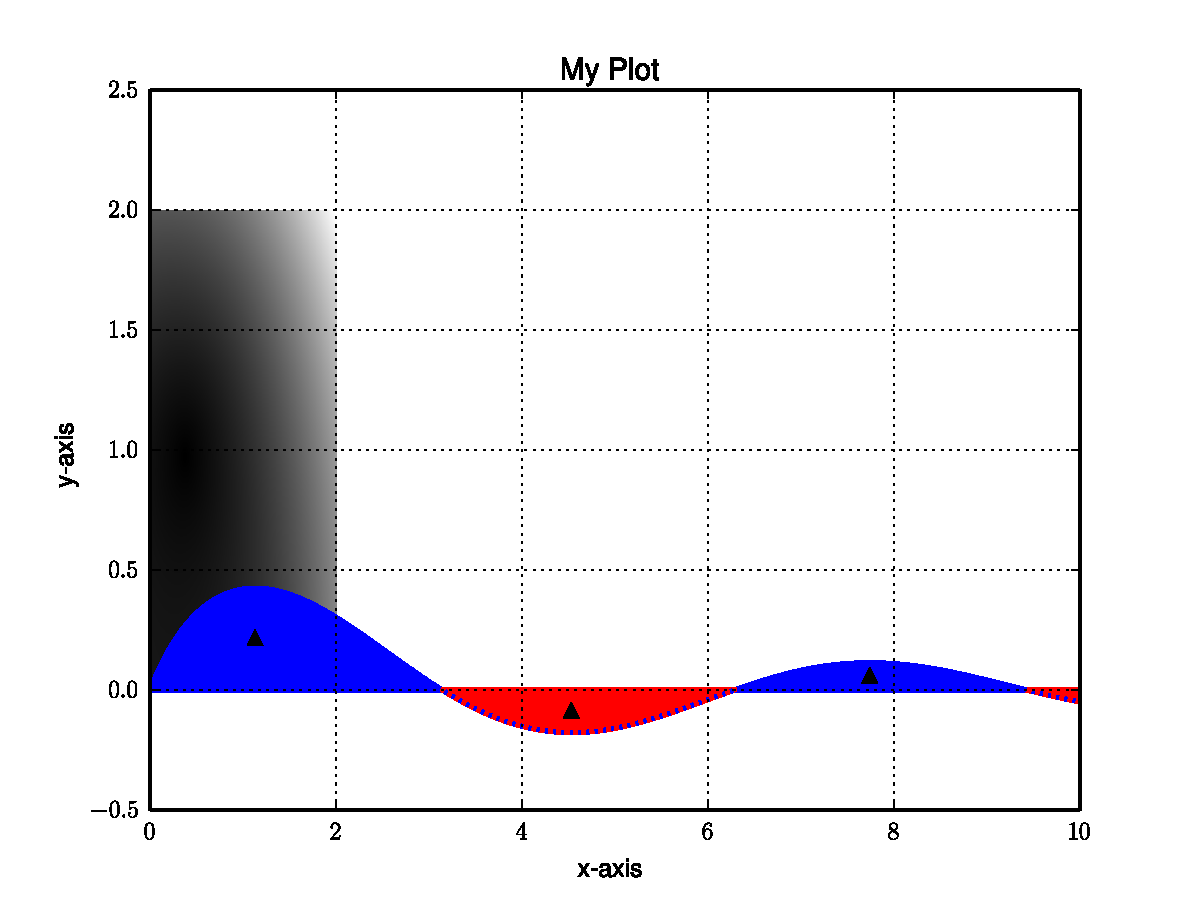
\includegraphics[width=\textwidth]{soln3.pdf}
\label{fig:problem3}
\end{figure}
\end{problem}
\end{comment}




\subsection*{Heatmaps}
A function from $\mathbb{R}^2$ to $\mathbb{R}$ is usually plotted as a surface in $\mathbb{R}^3$.
A \emph{heatmap} visualizes such a function in only two dimensions by assigning the output of the function to a color (instead of a height).
For example, Figure \ref{fig:pcmexample} uses a heatmap to graph $f(x,y) = \sin(x)\sin(y)$ on $[-6,6] \times [-6,6]$.

The plot in Figure \ref{fig:pcmexample} was created with the function \li{plt.pcolormesh()}.
To draw Figure \ref{fig:pcmexample}, we must first create a grid of points at which to evaluate $f$.
We do this with the function \li{np.meshgrid()}, which is explained in Figure \ref{fig:meshgrid}.

\begin{figure}
\begin{tikzpicture}[>=stealth', shorten <= .1cm,shorten >=.1cm, dot/.style=
	{circle,fill=black,minimum size=3pt,inner sep=0pt, outer sep=-1pt} ]

\foreach \x/\y in {0/0, 0/2, 0/4, 2/0, 2/2, 2/4, 4/0, 4/2, 4/4} 
	\node[draw, dot]at(\x,\y){};
\foreach \x/\y in {0/0, 0/1, 0/2, 1/0, 1/1, 1/2, 2/0, 2/1, 2/2} 
	\node[draw=none]at(\x*2-.5, \y*2+.3){(\x,\y)};

\foreach \x/\y in {0/0, 0/1, 0/2, 1/0, 1/1, 1/2, 2/0, 2/1, 2/2} 
	\node[draw=none]at(\x*.75+7, \y*.75+.1){\y};
\foreach \x/\y in {0/0, 0/1, 0/2, 1/0, 1/1, 1/2, 2/0, 2/1, 2/2} 
	\node[draw=none]at(\x*.75+7, \y*-.75+3.9){\x};

\draw[-, thick](6.7,-.25)--(6.7,1.95); 
\draw[-, thick](8.8,-.25)--(8.8,1.95);
\draw[-, thick](6.7,2.05)--(6.7,4.25);
\draw[-, thick](8.8,2.05)--(8.8,4.25);
\draw[-, thick](8.8,4.14)--(8.7,4.14);
\draw[-, thick](8.8,2.16)--(8.7,2.16);
\draw[-, thick](6.7,4.14)--(6.8,4.14);
\draw[-, thick](6.7,2.16)--(6.8,2.16);
\draw[-, thick](8.8,1.84)--(8.7,1.84);
\draw[-, thick](8.8,-.135)--(8.7,-.135);
\draw[-, thick](6.8,1.84)--(6.7,1.84);
\draw[-, thick](6.8,-.135)--(6.7,-.135);

\node[draw=none](X)at(6.3,.9){\texttt{Y}=};
\node[draw=none](y)at(6.3,3.15){\texttt{X}=};

\node[draw=none](point1)at(-.3, -.4){\texttt{x}=\big[0,};
\node[draw=none, node distance=2.35cm](point2)
	[right of=point1]{1,};
\node[draw=none, node distance=2cm](point3)
	[right of=point2]{2\big]};
\node[draw=none, rotate=270](point4)at(4.4,4.25)
	{\texttt{y}=\big[0,};
\node[draw=none, rotate=270, node distance=2.35cm](point5)
	[right of=point4]{1,};
\node[draw=none, rotate=270, node distance=2cm](point6)
	[right of=point5]{2\big]};



\end{tikzpicture}

\caption{This figure illustrates the function call \li{np.meshgrid(x, y)}, which returns the arrays \li{X} and \li{Y}. 
The returned arrays give the $x$- and $y$-coordinates of the points in the grid formed by \li{x} and \li{y}.}
\label{fig:meshgrid}
\end{figure}

\begin{lstlisting}
x = np.linspace(-6, 6, 401)
y = np.linspace(-6, 6, 401)
X, Y = np.meshgrid(x, y)
\end{lstlisting}
The arrays $X$ and $Y$ satisfy \li{(X[i,j], Y[i,j]) = (x[i],y[j])}.

Now we can evaluate $f(x,y)$ at each point in the grid and plot the result.
\begin{lstlisting}
f = np.sin(X) * np.sin(Y)
plt.pcolormesh(X, Y, f)
plt.pcolorbar()    # Show scale
plt.show()
\end{lstlisting}
This plot is shown in Figure \ref{fig:pcmexample}
\begin{figure}
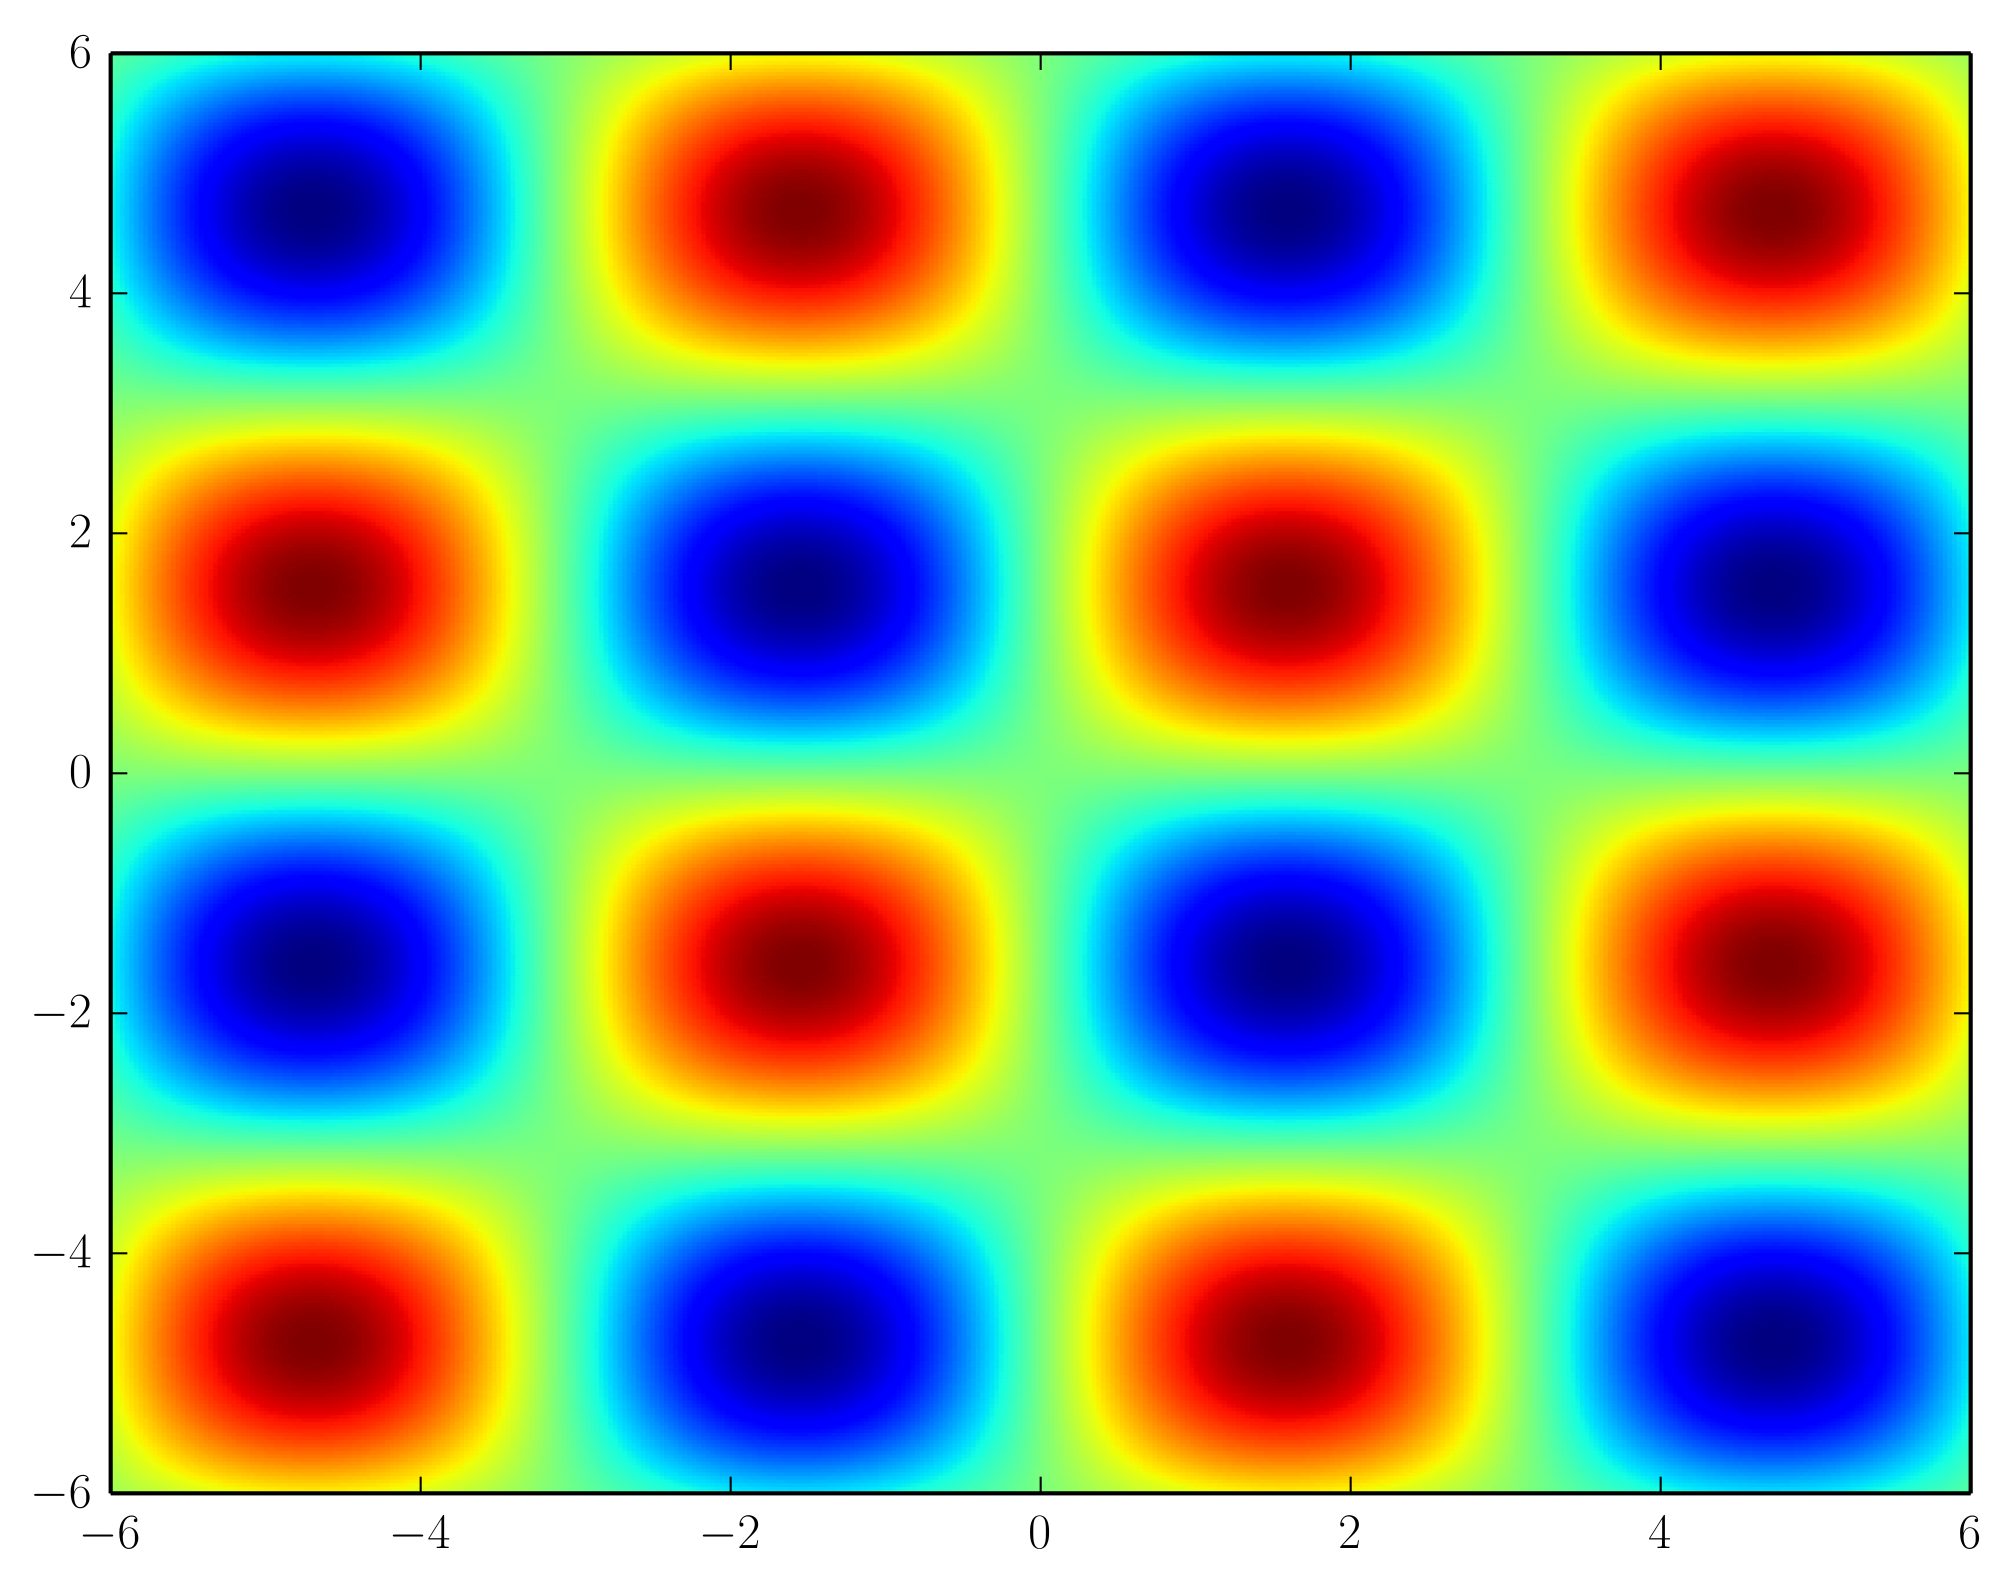
\includegraphics[width=.7\textwidth]{sinxsiny.png}
\caption{A heatmap of $f(x,y)=\sin\left(x\right)\times\sin\left(y\right)$ drawn by \li{plt.pcolormesh()}.}
\label{fig:pcmexample}
\end{figure}

\begin{comment}
\begin{problem} Use plt.pcolormesh to plot the absolute value of the function $x^3 +2x^2 -x +3$ on the complex plane with 0 $\leq$ \li{x} $\leq$ 2 and 0 $\leq$ \li{y} $\leq$ 2.
\emph{Helpful Hint}: First create your domain arrays, then convert these to a single array of complex variables to evaluate the function.

Your plot should look like Figure \ref{fig:pcolormesh}.

\begin{figure}[H]
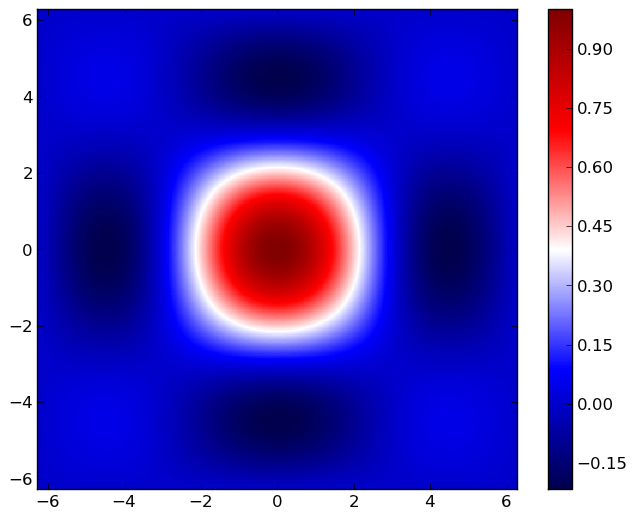
\includegraphics[width=\textwidth]{pcolor2.png}
\caption{Another example of a colorplot.}
\label{fig:pcolormesh}
\end{figure}
\end{problem}
\end{comment}

\begin{problem}\label{prob:heatmap}
\leavevmode
\begin{enumerate}
\item Plot the function $f(x,y) = \sin(x)\sin(y)/(xy)$ on $[-2\pi,2\pi] \times [-2\pi,2\pi]$. 
Include the scale bar in your plot.
\item Change the color scheme of your plot with the keyword argument \li{cmap='seismic'} in the call to \li{plt.pcolormesh()}. 
You can see a list of all possible color schemes at \url{http://matplotlib.org/examples/color/colormaps_reference.html}.
\item Change the limits on the $x$- and $y$-axes so that the plot is only over the domain $[-2\pi,2\pi] \times [-2\pi,2\pi]$.
\item Fix the aspect ratio of your plot so that it is a square using the line \li{plt.gca().set_aspect('equal')}.
\end{enumerate}
Your finished plot should look like Figure \ref{fig:heatmapProb}.

\begin{figure}[H]
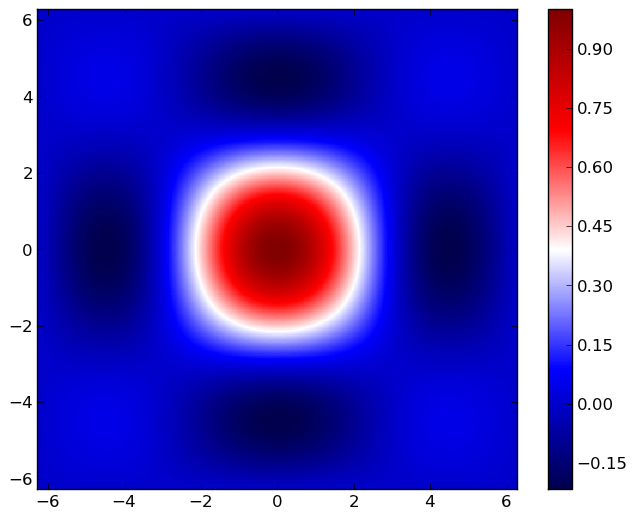
\includegraphics[width=.7\textwidth]{pcolor2.png}
\caption{Correct output for Problem \ref{prob:heatmap}.}
\label{fig:heatmapProb}
\end{figure}
\end{problem}

\begin{comment}

Matplotlib can also be used for 3D plotting. The following is an example
of how to use matplotlib to plot the function $z=\sin(x)\sin(y)$ with
both x and y ranging from -6 to 6. The resulting plot is shown in Figure
\ref{mpl:3dplot}. If you change the number of sample points used you
will notice that graphs look much nicer with large numbers of sample
points, but it will also take much longer for your computer to render
the image.

\begin{lstlisting} from mpl_toolkits.mplot3d import Axes3D from
matplotlib import pyplot as plt import numpy as np fig = plt.figure() ax
= fig.gca(projection='3d') x = np.linspace(-6, 6, 301) y =
np.linspace(-6, 6, 301) X, Y = np.meshgrid(x, y) Z = np.sin(X) *
np.sin(Y) ax.plot_surface(X, Y, Z) plt.show() \end{lstlisting}

\begin{figure} 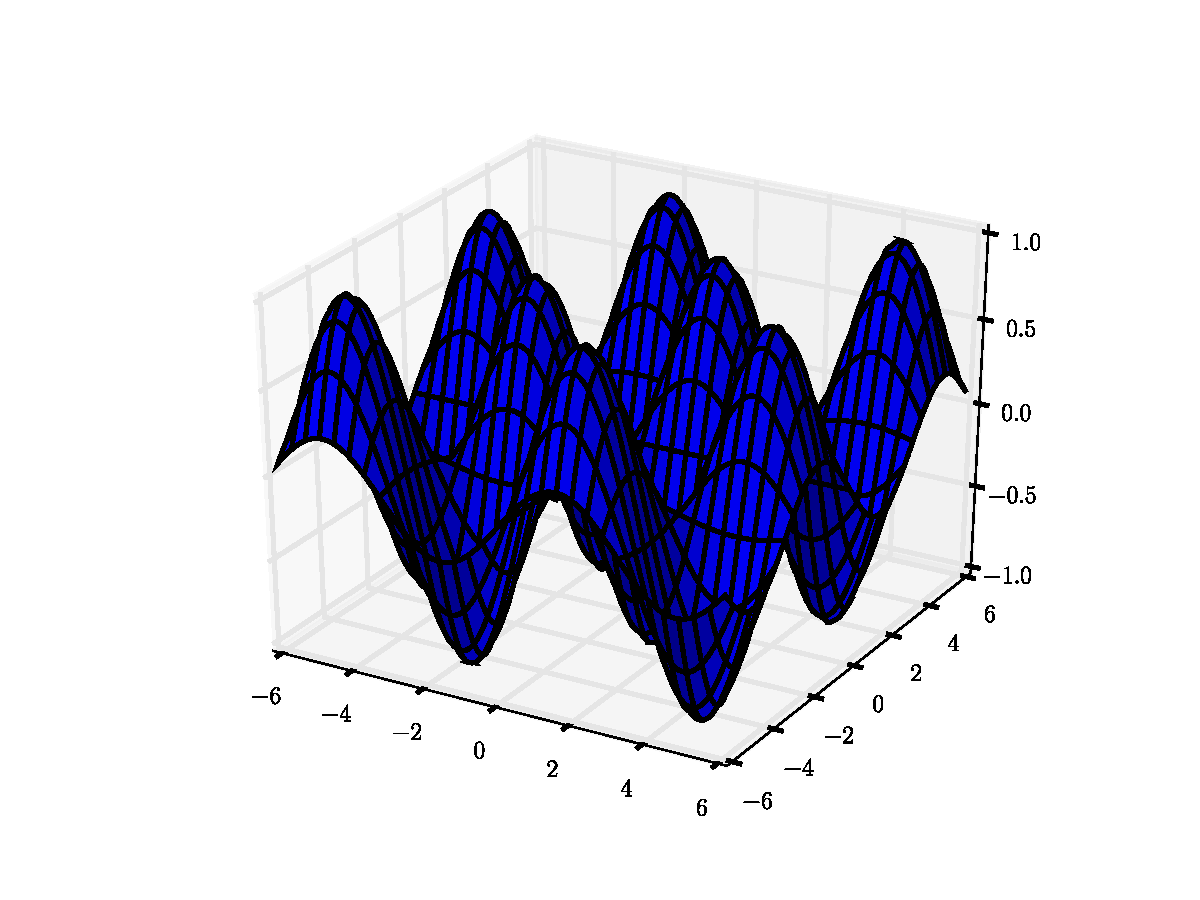
\includegraphics[width=\textwidth]{3dplot.pdf} \caption{A
3D plot of $\sin\left(x\right)\times\sin\left(y\right)$.}
\label{mpl:3dplot} \end{figure}

\begin{problem} Plot the function \begin{equation*}
\frac{\cos\left(\sqrt{x^2 + y^2}\right)}{\frac{x^2 + y^2}{10} + 1}
\end{equation*} on $[-10, 10] \times [-10, 10]$. \end{problem}


Matplotlib also allows us to make interactive graphs as follows:

% This example is largely based on one of the examples in the matplotlib
% docs. I have simplified it and changed the way the libraries are
% imported, but we could do a citation anyway.
%
\begin{lstlisting} import numpy as np from matplotlib import pyplot as
plt from matplotlib import widgets as wg ax = plt.subplot(111)
plt.subplots_adjust(bottom=.25) t = np.arange(0., 1., .001) a0 = 5. f0 =
3. s = a0 * np.sin(2 * np.pi * f0 * t) l = plt.plot(t, s)[0]
plt.axis([0, 1, -10, 10]) axfreq = plt.axes([.25, .05, .65, .03]) axamp
= plt.axes([.25, .1, .65, .03]) sfreq = wg.Slider(axfreq, 'Freq', .1,
30., valinit=f0) samp = wg.Slider(axamp, 'Amp', .1, 10., valinit=a0) def
update(val): amp = samp.val freq = sfreq.val l.set_ydata(amp * np.sin(2
* np.pi * freq * t)) plt.draw() sfreq.on_changed(update)
samp.on_changed(update) plt.show() \end{lstlisting} The resulting plot
is shown in Figure \ref{mpl:interact}.

\begin{figure} 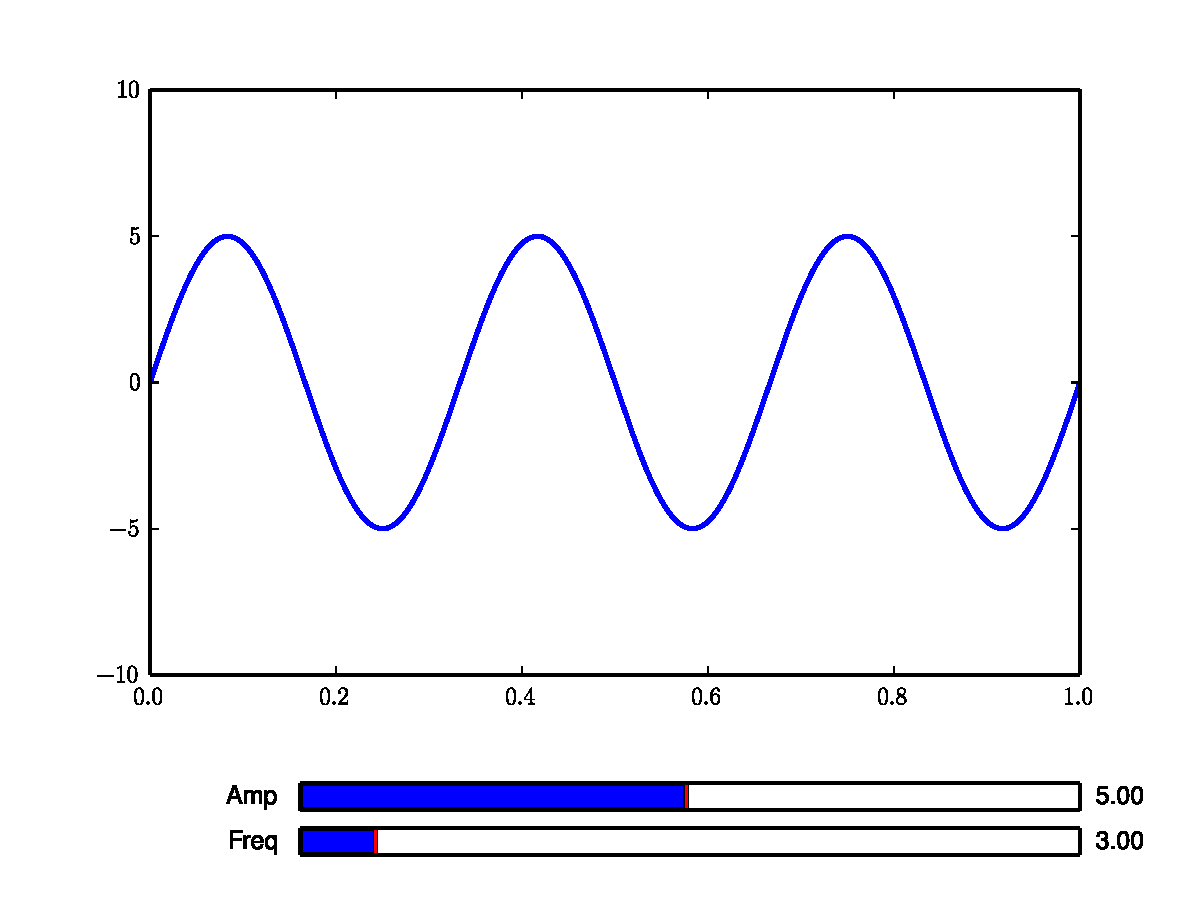
\includegraphics[width=\textwidth]{interact.pdf}
\caption{A snapshot of an interactive plot made using Matplotlib.}
\label{mpl:interact} \end{figure}

\begin{problem} Modify the code above to add a third slider to
manipulate the phase of the wave shown. Have it range from 0 to $2\pi$
and set the default value to zero. \end{problem}

\end{comment}

\subsection*{Other plots}
A \emph{histogram} is a way to visualize a 1-D data set, or list of values. 
A histogram is created by dividing up the range of the values into a finite number of intervals, or \emph{bins}.
Then, the number of values in each bin is added up.
Graphically, these totals are represented by bars whose length is equal to the number of values in the bin.

For example, suppose we randomly choose 20 integers between 1 and 10.
This code creates a histogram depicting how many of each number we chose.
Its output is in Figure \ref{fig:histogram}.

\begin{lstlisting}
x = np.random.randint(1, 11, 20)
plt.hist(x, bins=10, range=[.5, 10.5])
plt.show()
\end{lstlisting}

In this example our data set \li{x} consists of only integer values.
We created 10 bins in the range [.5, 10.5] so that each bin contains exactly one integer.

The function \li{plt.hist()} also returns some arrays, the first of which is a list of the total number of values in each bin.

We could also use a \emph{scatter plot} to visualize the random integers \li{x} that we generated in the previous example. 
The \li{matplotlib} function call \li{plt.scatter(x,y)} draws a scatter plot from two 1-D arrays \li{x} and \li{y} by plotting the points \li{(x[i], y[i])}.
As an example, the code below produces Figure \ref{fig:scatter}.

\begin{lstlisting}
t = np.linspace(1,20,20)
# The argument 's' specifies the marker size
plt.scatter(t, x, s=100)
plt.show()
\end{lstlisting}


\begin{figure}
\centering
\begin{subfigure}[t]{.49\textwidth}
\centering
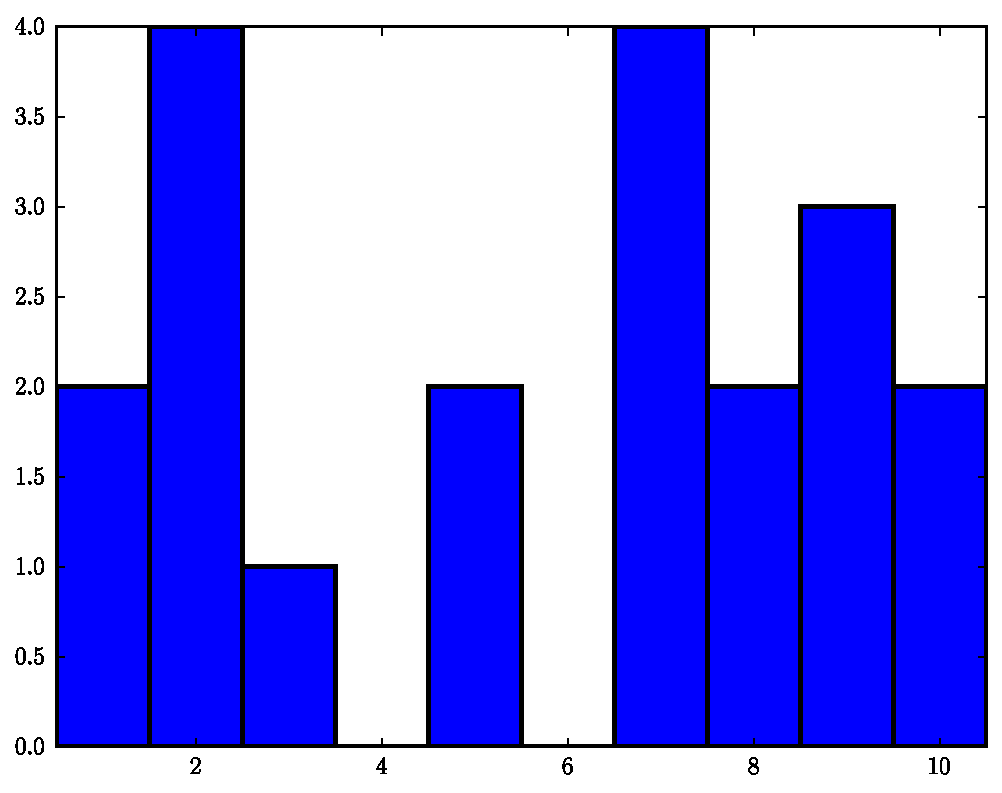
\includegraphics[width=\textwidth]{histogram.pdf}
\caption{A histogram.}
\label{fig:histogram}
\end{subfigure}
\begin{subfigure}[t]{.49\textwidth}
\centering
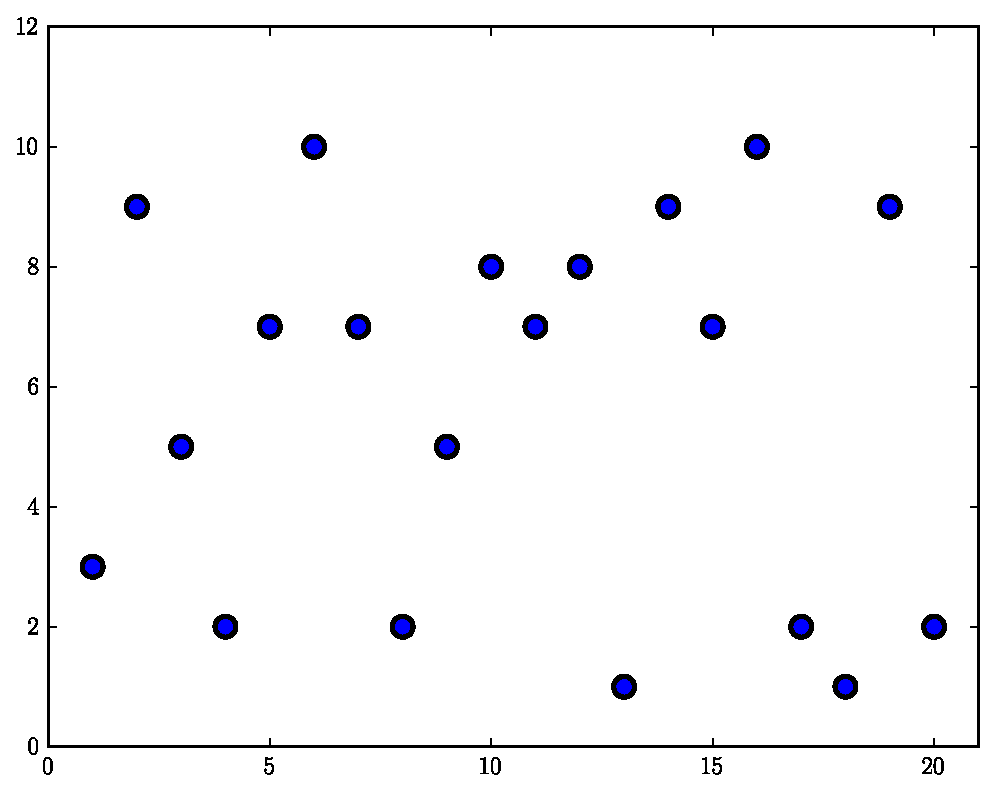
\includegraphics[width=\textwidth]{scatter.pdf}
\caption{A scatter plot.}
\label{fig:scatter}
\end{subfigure}
\caption{A scatter plot produced with \li{plt.scatter()} and a histogram produced with \li{plt.hist()}.}
\label{fig:otherplots}
\end{figure}


\subsection*{Subplots}
\emph{Subplots} are nonoverlapping plots arranged in a grid within a single figure (see Figure \ref{fig:subplots}).
In \li{matplotlib}, specify which subplot you wish to modify with with command \li{plt.subplot(numrows, numcols, fignum)}.
Here, \li{numrows} is the number of rows of subplots in the figure, \li{numcols} is the number of columns of subplots in the figure, and \li{fignum} is the index of the subplot you wish to modify.
This index starts at 1 and increments across rows first.

The following code draws Figure \ref{fig:subplots}.
\begin{lstlisting}
x = np.linspace(-np.pi, np.pi, 400)
y1 = np.sin(x)
y2 = np.cos(x)

# Draw the first subplot
plt.subplot(2, 1, 1)
plt.plot(x, y1)

# Draw the second subplot
plt.subplot(2, 1, 2)
plt.plot(x, y2)

plt.show()
\end{lstlisting}

\begin{figure}
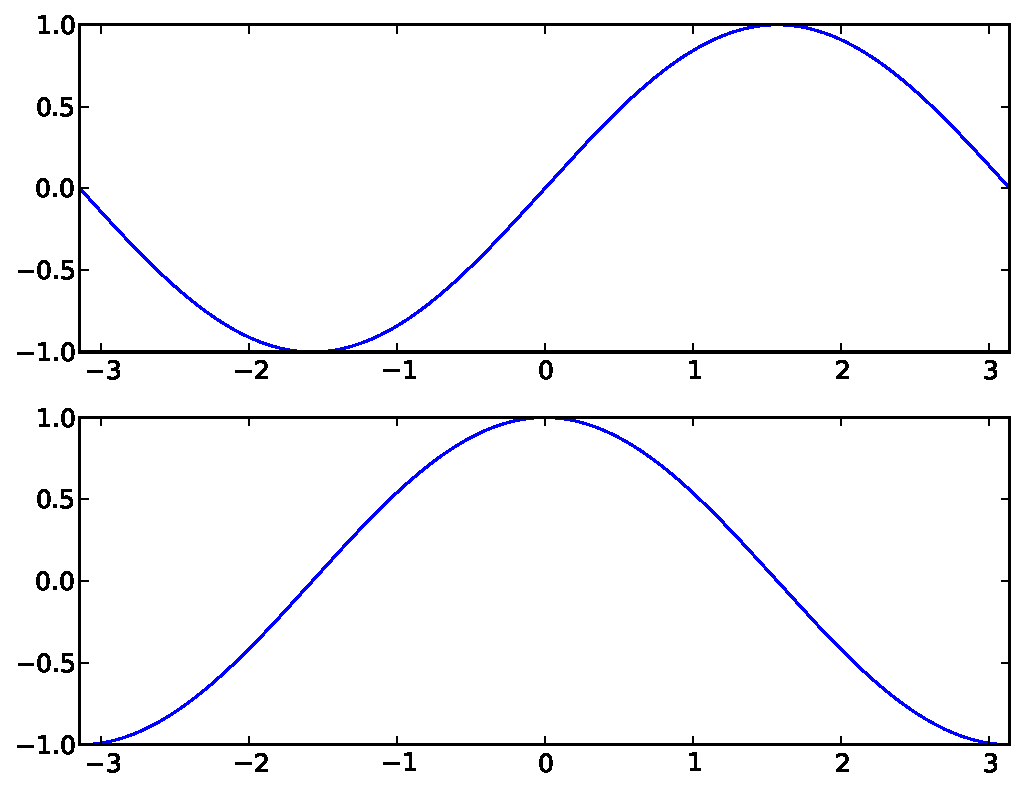
\includegraphics[width=.7\textwidth]{subplots.pdf}
\caption{The graphs of $\sin(x)$ and $\cos(x)$ as subplots in a single figure.}
\label{fig:subplots}
\end{figure}

\begin{problem}\label{prob:subplot}
Follow these steps to generate a plot similar to that in Figure \ref{fig:subplotProb}.
\begin{enumerate}
\item Generate 50 random numbers in the interval $[0,1)$ with the function \li{np.random.rand()}.
\item Create a plot with two subplots. 
In the first subplot, draw a histogram of your data with 5 equally-sized bins.
\item In the second subplot, 
\begin{enumerate}
\item Draw a scatter plot of your data. 
Use the integers 1-50 for the $x$-coordinates and use your data for the $y$-coordinates.
\item Plot a red horizontal line whose height is equal to the mean of your data.
\end{enumerate}
\end{enumerate}

\begin{figure}[H]
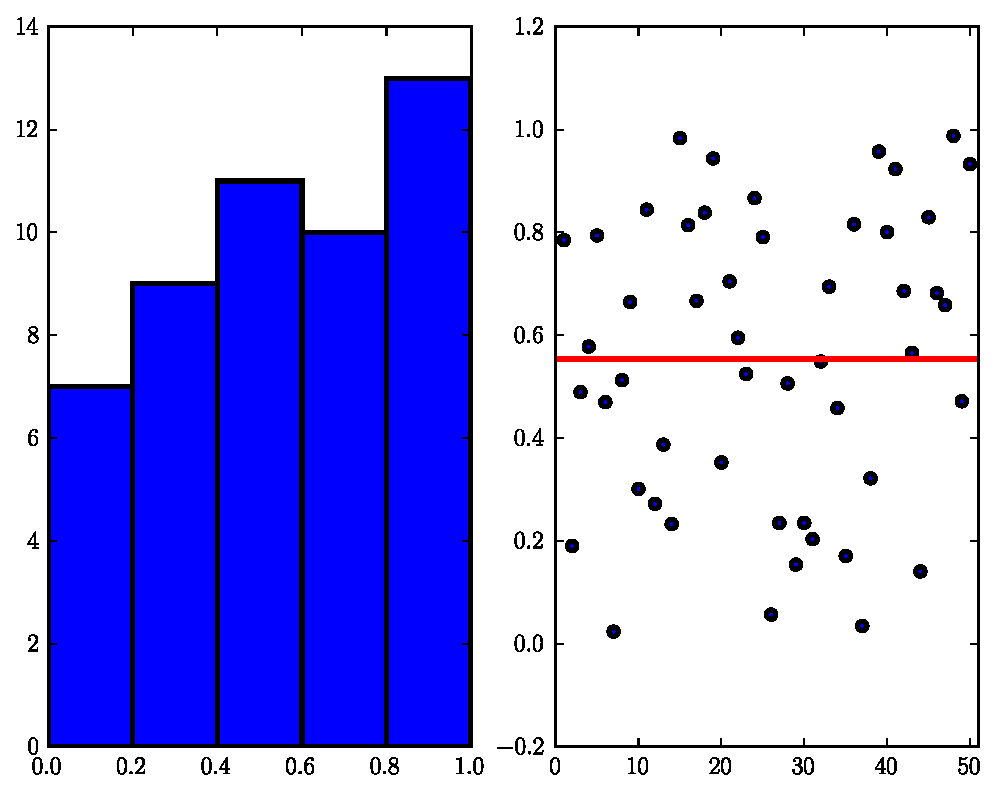
\includegraphics[width=.7\textwidth]{subplotProb.pdf}
\caption{Correct output for Problem \ref{prob:subplot}.}
\label{fig:subplotProb}
\end{figure}

\end{problem}


\begin{comment}
\begin{problem}
Make a plot with 4 subplots.
In the subplots place graphs of $e^x$, $sin(x)$, $cos(x)$, and $x^2$.
Plot each graph over the interval $(-\pi,\pi)$.
Title each graph accordingly and title the entire figure ``My Different Plots."
\end{problem}
\end{comment}

\begin{comment}
%Table \ref{mpl:basics}
\begin{table}
\begin{center}
\begin{tabular}{|l|p{7cm}|p{3cm}|}

    \hline

    Function & Description & Usage\\

    \hline

    \li{bar} & makes a bar graph & bar(left,height)\\

    \li{barh} & makes a horizontal bar graph & barh(bottom,width)\\

    \li{fill} & plots lines with shading under the curve & fill(x,y)\\

    \li{fill\_between} & plots lines with shading between two given y
    values & fill\_ between(x,y1, y2=0)\\

    \li{hist} & plots a histogram from data & hist(data)\\

    \li{pie} & make a pie chart & pie(x)\\

    \li{plot} & plots lines and data on standard axes & plot(x,y)\\

    \li{polar} & plots lines and data on polar axes & polar(theta,r)\\

    \li{loglog} & plots lines and data on logarithmic x and y axes &
    loglog(x,y)\\

    \li{scatter} & plots data, has more options for scatter plots than
    the plot function & scatter(x,y)\\

    \li{semilogx} & plots lines and data with a log scaled x axis &
    semilogx(x,y)\\

    \li{semilogy} & plots lines and data with a log scaled y axis &
    semilogy(x,y)\\

    \li{specgram} & make a spectogram from data & specgram(x)\\

    \li{spy} & plot the sparsity pattern of a 2D array & spy(Z)\\

    \li{triplot} & plot triangulation between given points &
    triplot(x,y)\\

    \hline

    \end{tabular}
    \end{center}
    \caption{Some basic functions in Matplotlib.}
    \label{mpl:basics}
    \end{table}


    \end{comment}

\section*{3-D plotting with Mayavi (Optional)}

Although \li{matplotlib} is capable of creating 3-D plots, Mayavi does it better. 
We will use Mayavi for all 3-D plots in these labs.
For information beyond what is found in this tutorial, see \url{http://docs.enthought.com/mayavi/mayavi/}.
To get started, import \li{mlab} from \li{mayavi}.
\begin{lstlisting}
from mayavi import mlab
\end{lstlisting}

The module \li{mlab} has many plotting functions.
We will introduce a few in this lab; for more see \url{http://docs.enthought.com/mayavi/mayavi/auto/mlab_helper_functions.html}.
You can also browse examples at \url{http://docs.enthought.com/mayavi/mayavi/auto/examples.html}.

\begin{comment}
\begin{table}
\begin{center}
\begin{tabular}
{|c|l|}
\hline
Function & Description \\
\hline
\li{barchart} & Produces 3D histogram-like plots\\
\li{contour3d} & Plots level surfaces of functions of three variables\\
\li{flow} & Creates a trajectory of particles following the flow of a vector field\\
\li{imshow} & Use a colormap to view a 2D array as an image\\
\li{mesh} & Plot a surface using \li{(x,y,z)} coordinates supplied as three 2D arrays\\
\li{plot3d} & Draws lines between points\\
\li{points3d} & Plots glyphs (like points) at the coordinates supplied\\
\li{quiver3d} & Generate 3D vector fields\\
\li{surf} & Plot a surface with a 2D array as elevation data\\
\hline
\end{tabular}
\end{center}
\caption{Some plotting functions in \li{mlab}.}
\label{table:mlab_functions}
\end{table}

All these functions can be ``tested" (which provides an example figure for the function) with the command:
\begin{lstlisting}
mlab.test_<plotting function>()
mlab.show()
\end{lstlisting}
Note that pressing tab after typing \li{mlab.test_} will provide a list of available commands and that, like matplotlib, we use the \li{show()} command to actually view our plot.

For example, to test the \li{fancy_mesh} function, we run the following:
\begin{lstlisting}
mlab.test_fancy_mesh()
mlab.show()
\end{lstlisting}


The result should resemble Figure \ref{fig:fancymesh}.

\begin{figure}
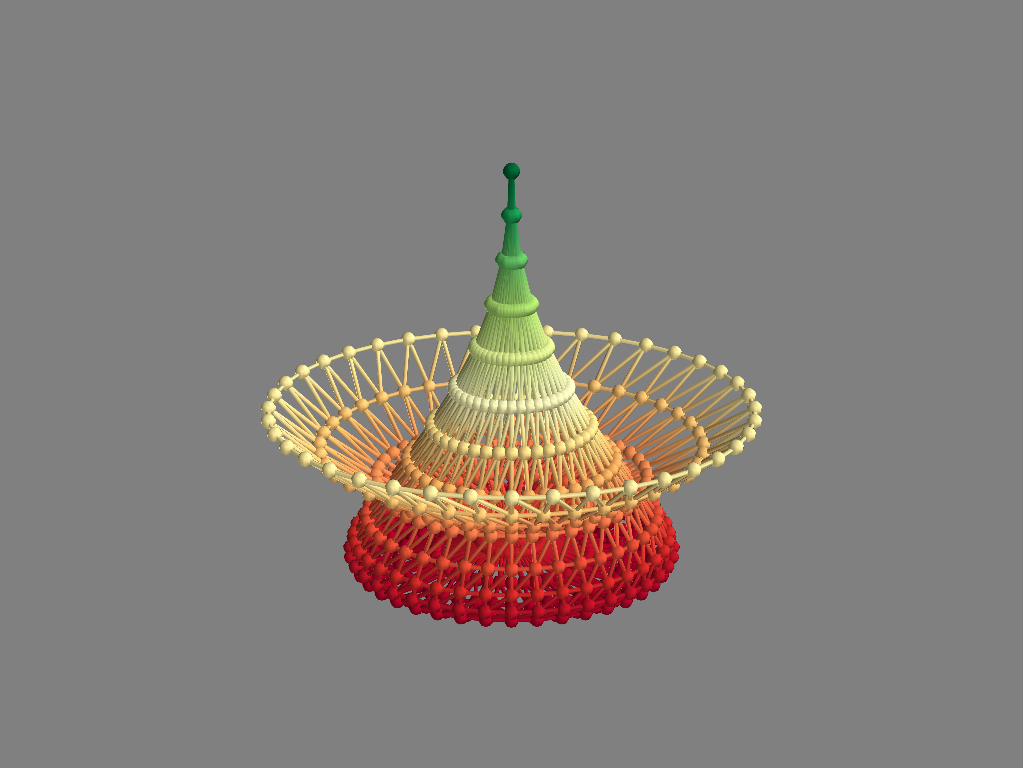
\includegraphics[width=\textwidth]{fancymesh.png}
\caption{An example of the fancy mesh plotting function}
\label{fig:fancymesh}
\end{figure}


In this lab, we will focus our attention on introducing the \li{mesh}, \li{plot3d}, and \li{points3d} functions.

Like matplotlib, \li{mlab} takes a set of data points and plots it.
However, instead of passing just \li{x} and \li{y} coordinates as we did in matplotlib, we also send \li{z} coordinates to produce a 3D plot.


\end{comment}

\subsection*{Lines}
The function call \li{mlab.plot3d(x,y,z)} plots the points \li{(x[i], y[i], z[i])} and connects them with straight lines.
The code below produces the flower in Figure \ref{fig:plot3d}

\begin{lstlisting}
num = np.pi/1000
pts = np.arange(0, 2*np.pi + num, num)
x = np.cos(pts) * (1 + np.cos(pts*6))
y = np.sin(pts) * (1 + np.cos(pts*6))
z = np.sin(pts*6/11)
mlab.plot3d(x, y, z)
mlab.show()
\end{lstlisting}

\begin{figure}

\includegraphics[width=.7\textwidth]{plot3d.png}
\caption{Sample output of \li{mlab.plot3d()}.}
\label{fig:plot3d}
\end{figure}


\subsection*{Points}
The function call \li{mlab.points3d(x,y,z)} plots the points \li{(x[i], y[i], z[i])}, but does not connect them. 
In the code below, the optional input array \li{s} defines a scalar for each point that modifies the color and size of the point.
The output is in Figure \ref{fig:points3d}.

\begin{lstlisting}
pts = np.linspace(0, 4 * np.pi, 30)
x = np.sin(2 * pts)
y = np.cos(pts)
z = np.cos(2 * pts)
s = 2+np.sin(pts)
# Adjust the keyword argument 'scale_factor' so all points are visible
mlab.points3d(x, y, z, s, scale_factor=.15)
mlab.show()
\end{lstlisting}

\begin{figure}
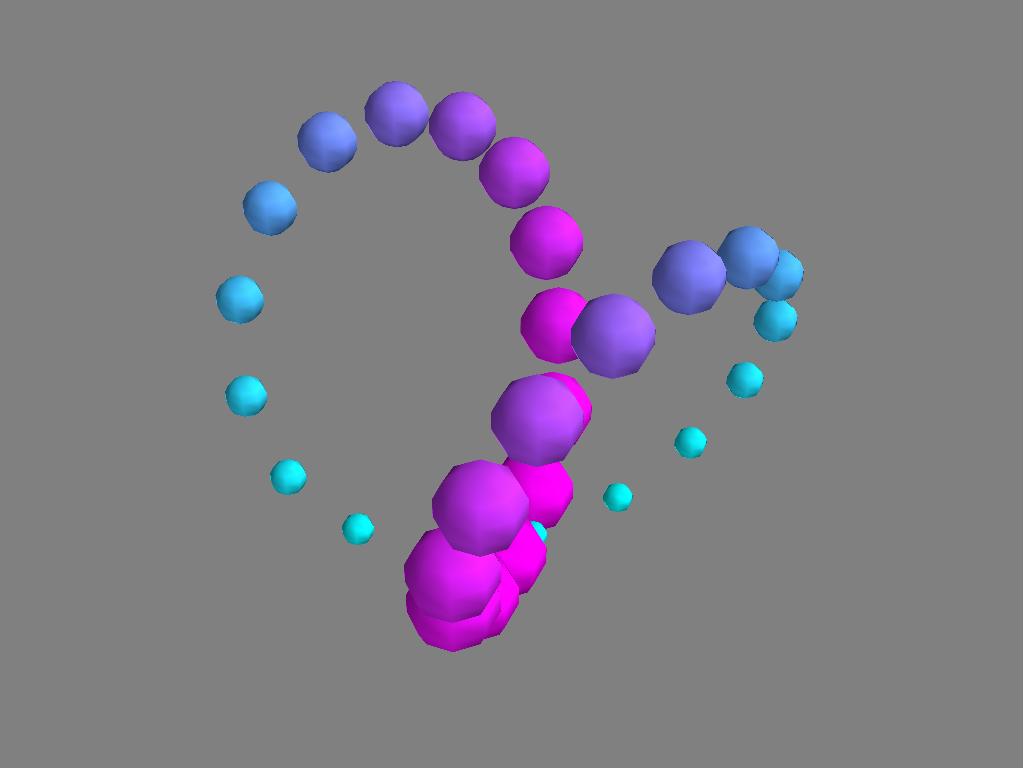
\includegraphics[width=.7\textwidth]{points3d.png}
\caption{Sample output of \li{mlab.points3d()}.}
\label{fig:points3d}
\end{figure}


\subsection*{Surfaces}
You can draw a surface in mayavi with \li{mlab.surf()}.
This function accepts three arrays, \li{X}, \li{Y}, and \li{Z}, where \li{X} and \li{Y} determine a grid of points similar to the output of \li{np.meshgrid()}.
The array \li{Z} gives the height of the surface at each of these points.

The output of \li{np.meshgrid()} is the transpose of what \li{mlab.surf()} expects.
To avoid confusion, use the function \li{np.mgrid()} instead.
This function uses the slicing syntax \li{[start:stop:step]} 
The code below produces the hyperbolic paraboloid in Figure \ref{fig:surf_example}.

\begin{lstlisting}
X, Y = np.mgrid[-4:4:0.025, -4:4:0.025]
Z = X**2/4-Y**2/4
mlab.surf(X, Y, Z, colormap='RdYlGn')
mlab.show()
\end{lstlisting}


\begin{figure}
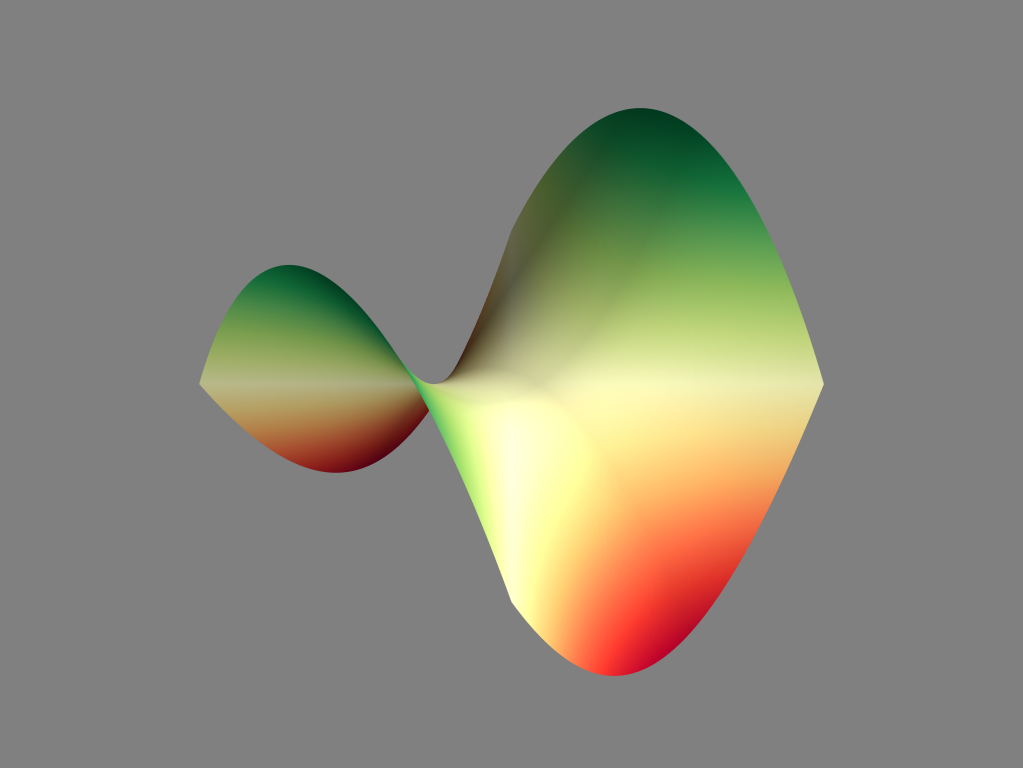
\includegraphics[width=.7\textwidth]{mesh_example.png}
\caption{Sample output of \li{mlab.surf()}.}
\label{fig:surf_example}
\end{figure}

The plotting functions in Mayavi allow you to specify the color of a plot, either as a solid color or with a varying colormap.
For example, the plot in Figure \ref{fig:surf_example} uses the colormap \li{'RdYlGn'}.
For a list of all colormaps in Mayavi, see \url{http://docs.enthought.com/mayavi/mayavi/mlab_changing_object_looks.html}.


%TODO: this problem is copied from https://github.com/enthought/mayavi/blob/master/examples/mayavi/mlab/canyon.py.
% we either need to cite this (and thus give the solution) or find a different problem.
\begin{comment}
\begin{problem}\label{prob:grand_canyon}
Provided Grand Canyon topological radar data from NASA, do the following.

\begin{itemize}
\item Reshape the data to be 3601x3601.
\item Cast the data type as \li{float32}.
\item Slice the data, taking the first 1000 rows and columns 900-1900.
\item There is some missing data, so set the minimum of your data equal to the minimum of the the positive data points.
\item Preset the figure using the following commands: \li{mlab.figure(size=(400,320)}, \li{bgcolor = (.16, .28, .46))}
\item Now plot with \li{mlab.surf}, using the colormap \li{gist_earth}, with a \li{warp_scale=.2}, \li{vmin=1200}, and \li{vmax=1610}.
\item Take a smaller view of the canyon using \li{mlab.view(-5.9, 83, 570, [5.3, 20, 238])}.
\end{itemize}

This should produce Figure \ref{fig:GrandCanyon}

\begin{figure}[H]
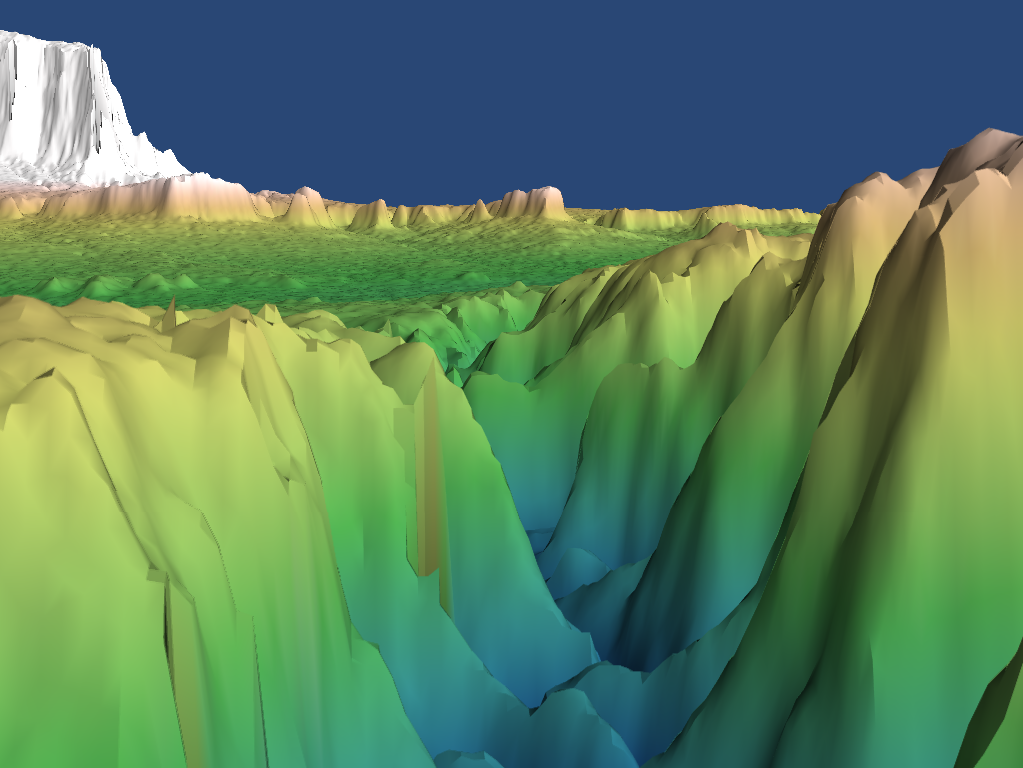
\includegraphics[width=.7\textwidth]{GrandCanyon.png}
\caption{Correct output for Problem \ref{prob:grand_canyon}.}
\label{fig:GrandCanyon}
\end{figure}

\end{problem}
\end{comment}

